\documentclass[onecolumn, draftclsnofoot, 10pt, compsoc]{IEEEtran}
\usepackage{listings}
\usepackage{url}
\usepackage{graphicx}
\usepackage{underscore}
\usepackage[bookmarks=true]{hyperref}
\usepackage[utf8]{inputenc}
\usepackage[english]{babel}
\usepackage{pdflscape}
\usepackage{pdfpages}
\usepackage{caption}
\usepackage{geometry}
\usepackage{booktabs}
\usepackage{multirow}
\geometry{letterpaper, margin=0.75in}

\hypersetup{
    pdftitle={Software Requirement Specification},    % title
    pdfauthor={CS USLI TEAM},                     % author
    pdfsubject={TeX and LaTeX},                        % subject of the document
    pdfkeywords={TeX, LaTeX, graphics, images}, % list of keywords
    colorlinks=true,       % false: boxed links; true: colored links
    linkcolor=blue,       % color of internal links
    citecolor=black,       % color of links to bibliography
    filecolor=black,        % color of file links
    urlcolor=purple,        % color of external links
    linktoc=page            % only page is linked
}%
\def\myversion{1.0}
\date{}

\usepackage{hyperref}
\begin{document}
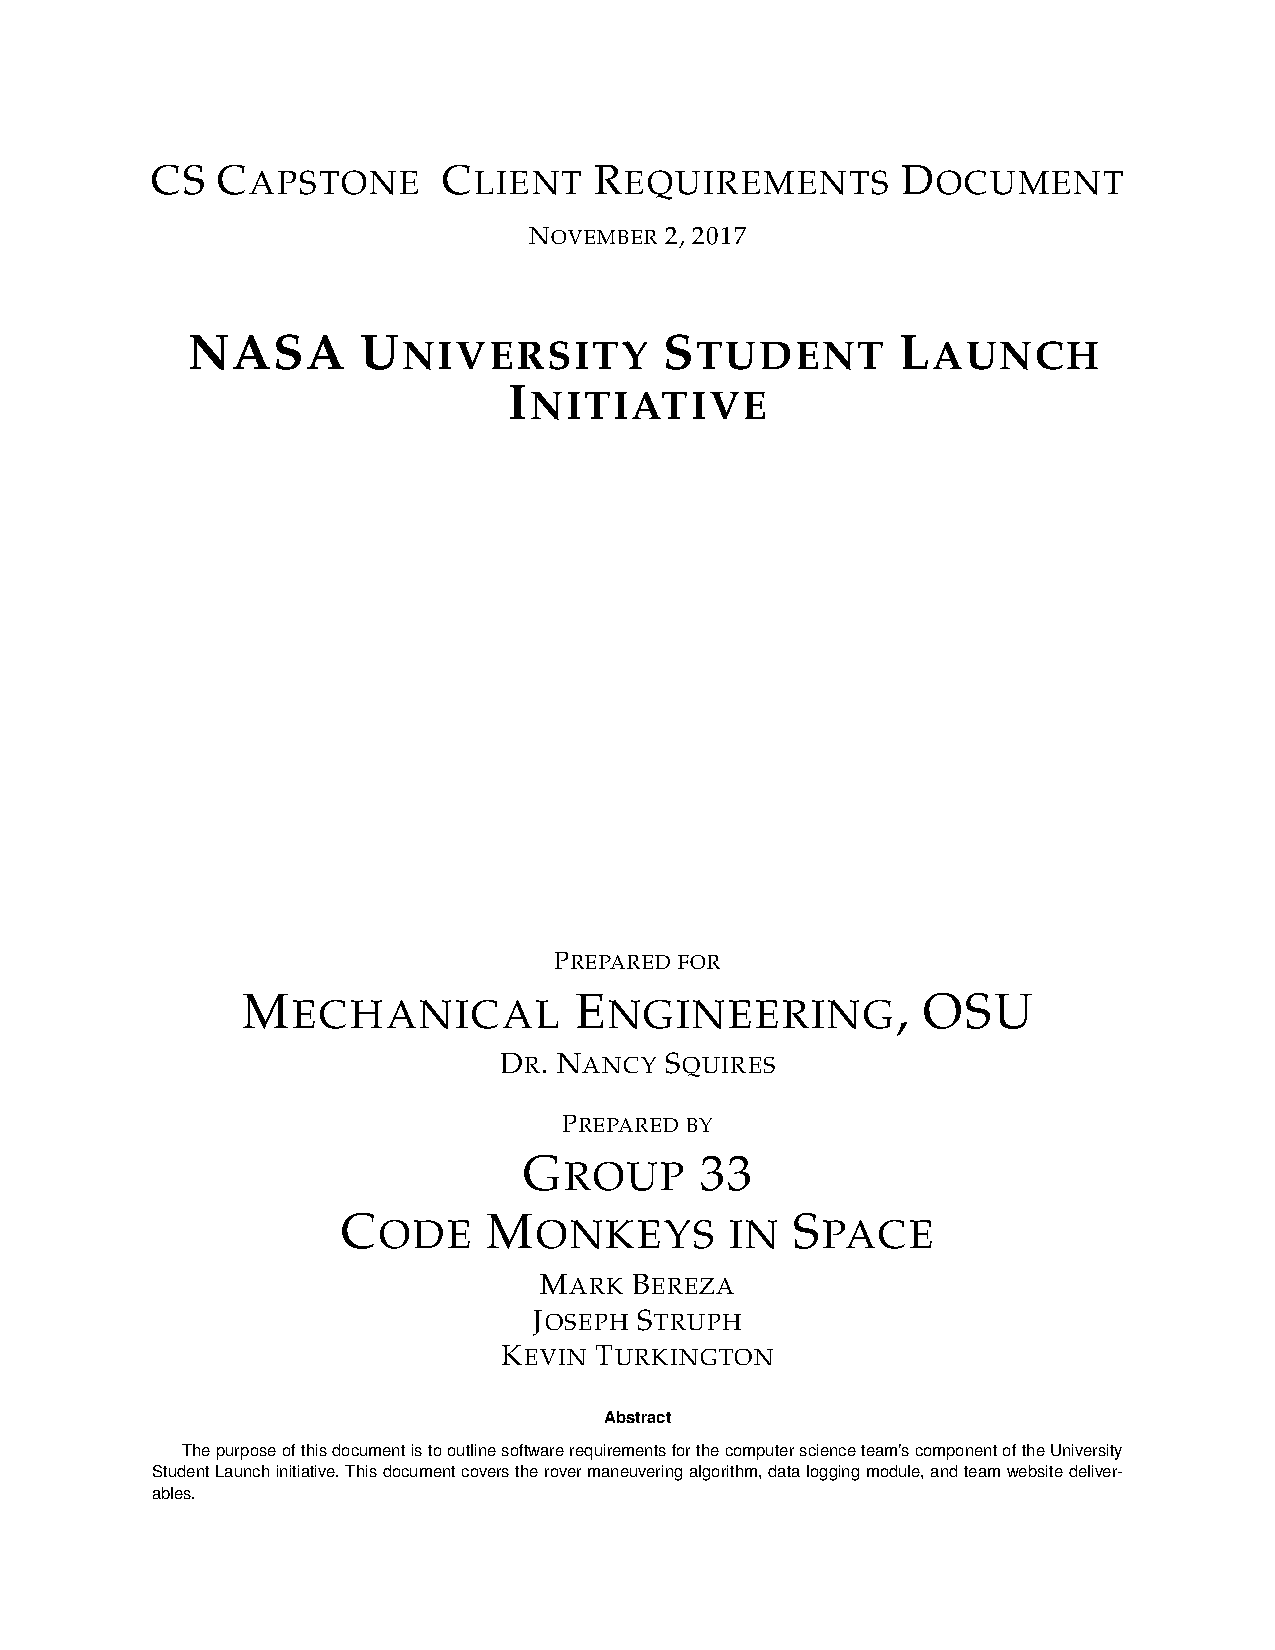
\includepdf{titlepage.pdf}
\tableofcontents

\section{Revision History}
\begin{table}[h]
\centering
\caption{Document Revision History Table}
\label{table:Revision History}
\begin{tabular}{@{}lllp{12cm}@{}}
\toprule
\textbf{Revision}    & \textbf{Date}            & \textbf{Sections}  & \textbf{Description}                                                                                                                                             \\ \midrule
1.0                  & 11/2/17                  & All               & Document creation                                                                                                                                                \\ \midrule
1.1 & 2/10/18 & 2.3, 4.2, 5.1, 5.2, 7.2 & \vspace{-15pt} \begin{itemize} \item Rover now using sound localization system instead of GPS. \item Removed the driver code/data collection aspect of the data logger to reflect that it has been taken up by a different subteam. \item Changed microcontroller for data logger from BeagleBone Black to Teensy to reflect changes made my team.\item Adding requirements for Design Review and Latex templates \end{itemize} \vspace{-15pt} \\ \bottomrule
\end{tabular}
\end{table}

\section{Introduction}

\subsection{Purpose}
The purpose of NASA's USLI is to construct and launch a rocket that will go at least a mile above ground, safely land, and deploy a rover capable of autonomous movement that will deploy solar cells after moving at least five feet from the rocket.

The CS students on OSU's USLI team are responsible for designing, implementing, and testing all software necessary to accomplish this task. 
This will include rover motor control and obstacle avoidance, graphical representation of test flight data, and creation/maintenance of a website hosting project information and deliverables.

\subsection{Document Conventions}
\subsubsection{Acronym Definitions}
\begin{tabular}{rl}
USLI: & University Student Launch Initiative\\
RMA: & Rover Maneuvering Algorithm \\
DLM: & Data Logging Module\\
PDR: & Preliminary Design Review\\
CDR: & Critical Design Review\\
FRR: & Flight Readiness Review\\
PLAR: & Post Launch Assessment Review\\
\end{tabular}

\subsection{Intended Audience and Reading Suggestions}
This document is intended for project stakeholders, USLI Team members, and anyone interested in the software component of the USLI rover experiment. This document is also meant for the NASA adjudicators and advising engineers. USLI team members and interested students may find the Overall Description and Systems Features sections most pertinent. On the other hand, project stakeholders and NASA advisors may find the System Features and Nonfunctional Requirements pertinent.

\subsection{Project Scope}
For a detailed description of the project's scope, please refer to the \href{https://github.com/OSU-USLI-18/Payload-Software/tree/master/capstone-documentation/33_problem_statement}{problem statement document} located on OSU USLI's software GitHub repository.

\subsection{References}
2018 NASA Student Launch Handbook: Colleges and Universities. Nasa, 2018. Web. Nasa.gov.

\section{Overall Description}

\subsection{Product Perspective}
This requirements document details the creation of several new software components to be used in the overall USLI mission profile and launch event. Specifically, these components include rover software, avionics software, and a team website. The overall mission profile concerns itself with the design, construction, testing, and launcing of a vehicle that will travel a distance of 5280 feet above ground level, safely land, and deploy the aforementioned payload after landing, which will then deploy solar cells. The payload software fits into this profile by facilitating autonomous movement and solar cell deployment. The avionics software fits into this profile by providing the team with useful flight data for testing purposes, The team website fits into this mission profile by being the medium through which design documents and other competition deliverables are communicated to NASA. Refer to the figure below for a visual overview of the mission profile:\\ \\
\begin{minipage}{\linewidth}
\begin{center}
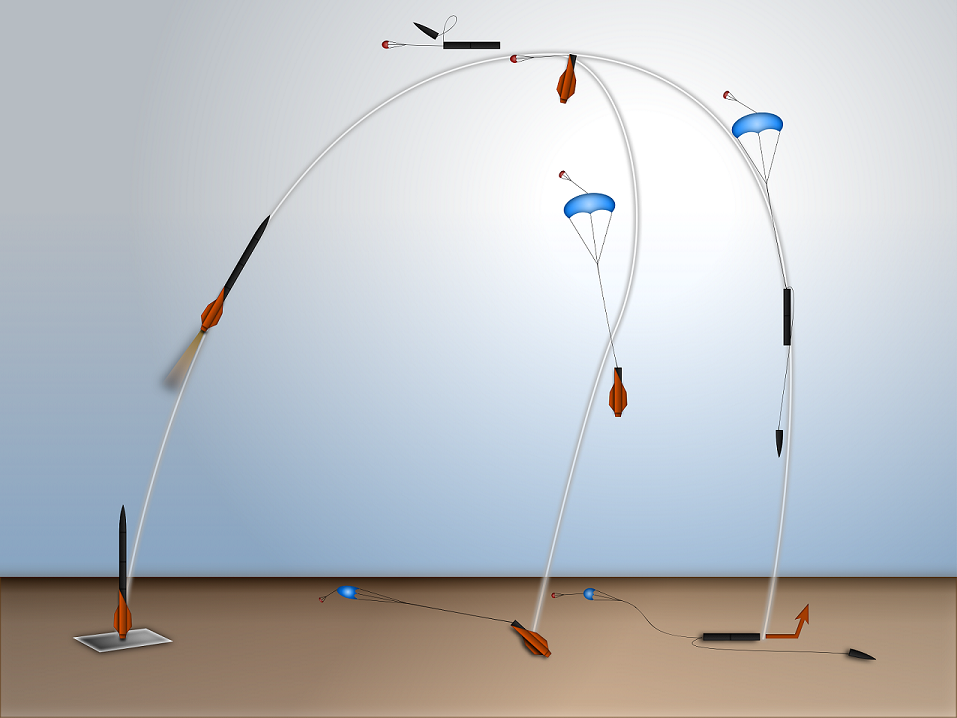
\includegraphics[width=\textwidth]{mission-profile}
\captionof{figure}{Planned trajectory and stages of the final rocket launch.}
\end{center}
\end{minipage}

\subsection{Product Functions}
\begin{itemize} 
\item Autonomously maneuver a rover away from the launch vehicle. 
\item Graphical representation of in-flight data.
\item Maintain a website detailing project information and hosting all competition deliverables.
\end{itemize}

\subsection{User Classes and Characteristics}
The primary users of the aforementioned products will be the project stakeholder and USLI team members who rely on these components for a successful launch, competition information communication, and favorable competition scoring. Secondary users include the NASA adjudicators and engineers who review the design and performance of the rover, rocket, and website for the competition. The largest user class are students and community members, who will rely on the website for team outreach information.

\subsection{Design and Implementation Constraints}
Hardware limitations are the biggest constraint for both the rover and avionics software. The OSU USLI team is comprised of multiple sub teams and all mechanical and electrical design decisions fall under separate sub teams comprised of mechanical and electrical engineering students. Since hardware constraints are almost always more constrictive than their software counterparts, the software generated by the computer science subteam must adapt to limitations imposed by the electrical and mechanical designs generated by the other subteams. In particular, the rover software created by Code Monkeys in Space must be compatible with and run on the microcontroller selected by the ECE and ME students. On the other hand, there are other constraints on the software arising from the requirements laid out in the USLI handbook provided by NASA, which demands that rover movement is autonomous and that website delivarables are accessible in PDF format and using minimal clicks from the home page. These different constraints will drive the software development.

\subsection{User Documentation}
User documentation will be available on the \href{http://osuusli.com/}{team website}, detailing design review repots and presentations, team structure, and educational outreach resources. Source code will be made available via the team's \href{https://github.com/OSU-USLI-18/Payload-Software}{GitHub repository}.

\subsection{Assumptions and Dependencies}
Due to the multi-stage nature of the launch, the software subteam must assume several minimal hardware requirements will be met by the subteams responsible for their successful implementation. In particular:
\begin{enumerate}
\item The launch vehicle will successfully launch and reach an altitude of roughly 5280 feet.
\item The launch vehicle will safely land.
\item The payload will successfully be ejected from the rocket frame after landing.
\item The microcontroller will be powered on after ejection.
\item The rover will have sufficient battery life after ejection to facilitate running the microcontroller, sensors, and motors long enough to move the required distance.
\item The motors will be capable of moving the rover after ejection.
\end{enumerate}

These baseline assumptions are unavoidable from the perspective of the software subteam because if any of them are not met during the final launch, no amount of software will address the underlying problem.

\section{External Interface Requirements}

\subsection{User Interfaces}
The only user interface for this project is the team website, which must be capable of displaying a variety of information about the comptetion, the vehicle design, and the team itself to a variety of audience types in an interactive way. The rover software does not feature a user interface because it must function autonomously. The avionics software will also lack a user interface because it will simply display flight data in a static way.

\subsection{Hardware Interfaces}
Both the Raspberry Pi and Teensy microcontrollers will communicate with peripheral sensors whose purpose is to provide information about the vehicle (temperature, pressure, acceleration) or its surroundings (distance from objects, altitude). The data logging module will take serial input from peripheral sensors, and output data to the ground station. The Raspberry Pi will take serial input from peripheral sensors, and output signals to control the rover's motors.

\section{System Features}

%%%% ROVER %%%%%%%

\subsection{Rover Maneuvering Algorithm (RMA)}
\subsubsection{Description and Priority}
Overall the highest priority for the software team is the rover payload itself.
The algorithm running on it will be used to control all movement of the rover without any human interaction through the use of onboard sensors such as sonar, microphone, and gyroscopes.
The main goal of the RMA is to allow the rover to move five feet from any part of the rocket body (excluding parachute/tethers) and deploy solar panels afterwards.

\subsubsection{Stimulus/Response Sequences}
The competiton rules only allow for a single button press to trigger rover deployment. However, ejection of the rover is a hardware-specific system and, as such, there are no human interaction sequences or user input for the rover.

\subsubsection{Functional Requirements}
\begin{itemize}
\item The rover will operate autonomously after the single button press for payload deployment.
\item The rover will move at least five feet from the rocket's land site before deploying solar cells.
\item The rover will drive its required distance without getting stuck on any obstacle for more than 15 minutes.
\item The rover will be tested in a real-world environment similar in terrain to the launch site before the competition in April.
\item The rover will have an escape maneuver in the event of stall current or a detected stoppage.
\end{itemize}

\subsubsection{Stretch Goals}
\begin{itemize}
\item All code will compile without errors or warnings before deployment to the rover.
\item All code deployed to the rover will have at least 90\% test coverage.
\item The rover will be able to continue to operate in the event of lost or diminished sensor functionality.
\end{itemize}

%%%% DATA LOGGING MODULE %%%%%%

\subsection{Avionics and Data Logging Module (DLM)}
\subsubsection{Description and Priority}
The next highest priority for the software subteam concerns the display of avionics information for the rocket after sensors have recorded various streams of data during test flights.
The rocket will be equipped with, at a minimum, an altimeter for elevation measurements, 9 degrees of freedom IMU, barometer, and a GPS sensor. Information from this data logger must be displayed in a human-readable fashion. 
\subsubsection{Stimulus/Response Sequences}

\subsubsection{Functional Requirements}
\begin{itemize}
\item Software will be written to convert the rockets logged data into a graphical representation.
\end{itemize}
\subsubsection{Stretch Goals}
\begin{itemize}
\item Data displayed at the ground station will accurately filter out signal and sensor noise.
\end{itemize}

%%%% WEBSITE %%%%%%%%%%%

\subsection{USLI Team Website}
\subsubsection{Description and Priority}
The website will be fairly minimalistic in appearance and hosted on the custom domain \href{http://osuusli.com/}{osuusli.com}. Most of the content will be contained on the home page and the site itself will be implemented using a template. The site will contain, at a minimum:
\begin{itemize}
\item The team name and logo (once available)
\item A list of all participants in the project
\item A brief description of the project and its goals
\item Download links for all project deliverables
\item A visual time line of important events and deadlines
\end{itemize}
Additionally, the site will:
\begin{itemize}
\item Run without errors
\item Be publically accessible
\item Allow users to download PDFs for all deliverables before their due date (as specified by NASA)
\end{itemize}
\subsubsection{Stretch Goals}
\begin{itemize}
\item Add a section for educational outreach and team photos.
\item Facilitate live viewing of the rocket's launch.
\item Maintain a social media presence for the team. 
\end{itemize}

\section{Nonfunctional Requirements}

\subsection{Software Quality Stretch Goals}
\begin{itemize}
\item All rover and avionics software changes to the master branch will only be made after review and approval from at least one team member (not the one requesting the change).
\item Changes to the rover or avionics master branches will require that all test cases are passing for the incoming branch.
\item The team will utilize Continuous Integration (CI) during the development of the software for the rover and avionics.
\item All software written for the rover will follow a single coding style.
\end{itemize}

\section{Other Requirements}
\subsection{Education Outreach}
\subsubsection{Description and Priority}
The goal of reaching 200 people over the course of the competition, a minimum requirement outlined in the USLI handbook, will be reached through a combination of various strategies. While the team will try to meet and exceed this number, the quality and intent behind the outreach is an equally important consideration. Outside of the K-12 requirement, the project sponsor would like to foster continued interest in projects like this at OSU from the AIAA (The American Institute of Aeronautics and Astronautics) club and students in the College of Mechanical Engineering. This aspect of the project is just as important as any other requirement, as it is a major part of the competition's scoring and one of NASA's primary motivations for hosting this competition in the first place. 

\subsubsection{Functional Requirements}
\begin{itemize}
\item Each member of the core team will volunteer to take an active role in educational outreach for at least two separate months between now and the competition's conclusion in April.
\item The team as a whole will reach at least 200 people before the competition's conclusion.
\end{itemize}
\subsubsection{Stretch Goals}
\begin{itemize}
\item Code Monkeys in Space will lead a visual programming language lesson for elementary school students using Scratch or Code.
\item Code Monkeys in Space will lead a visual programming or simple JavaScript lesson to middle school students.
\end{itemize}

\subsection{Design Review and Latex Templates}
\subsubsection{Description and Priority}
The design review documents: Preliminary Design Review, Critical Design Review, Flight Readiness Review, and Post Launch Assessment Review are worth 65\% of total competition points making them more important to the teams score than the points of both the rover and website combined. Due to this the CS team will assist the team in formatting, editing, and designing Latex templates and documents for the competition. 
\subsubsection{Functional Requirements}
\begin{itemize}
\item The CS team will create a Latex template for the USLI team to use for NASA design review document submissions.
\item The CS team will assist in editing and formatting of Latex documents for NASA design review.
\item The CS team will format figures, tables, and equations in Latex sourced from other USLI team members word and excel document submissions.
\item The CS team will compile and format USLI team members individual contributions to create one design document for the entire team.
\end{itemize}

\begin{landscape}
\section{Appendix}
\subsection{Gantt Chart}
\thispagestyle{empty}
\vspace*{\fill}
\noindent
\hspace*{-\oddsidemargin}%
\makebox[0pt][l]{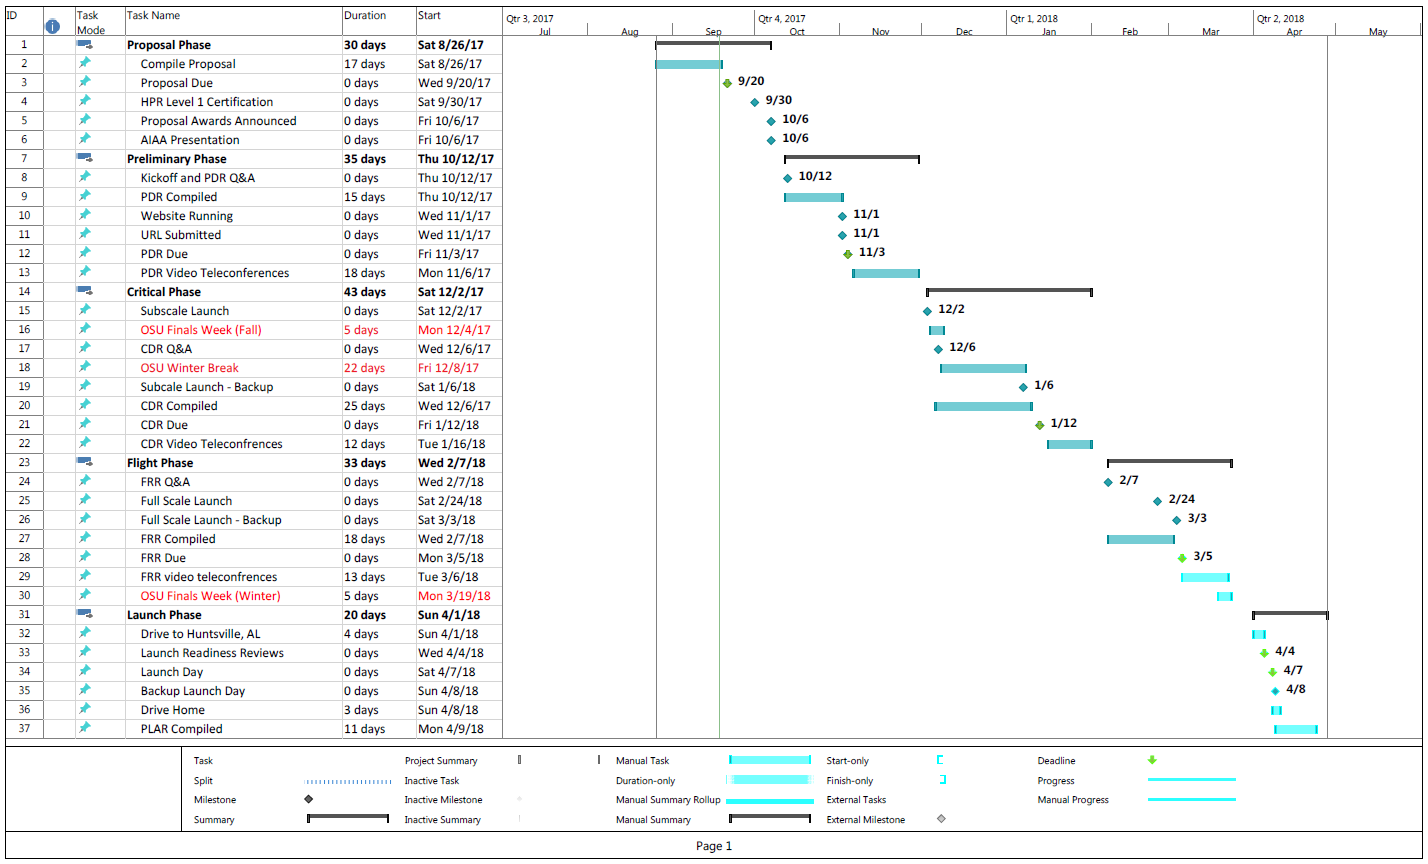
\includegraphics[width=1.28\textwidth]{GanttChart}}
\vspace*{\fill}
\vfill
\raisebox{-10pt}{\makebox[\linewidth]{\thepage}}
\end{landscape}

\end{document}
